\documentclass[conference]{IEEEtran}
\usepackage{newtxtext,newtxmath}
\usepackage{graphicx}
\usepackage{booktabs}
\usepackage{array}
\newcolumntype{L}[1]{>{\raggedright\arraybackslash}p{#1}}
\usepackage{amsmath}
\usepackage{xcolor}
\usepackage{tikz}
\usetikzlibrary{positioning,arrows.meta}
\usepackage[hidelinks]{hyperref}
\usepackage{url}

\newcommand{\id}[1]{\texttt{#1}}
\renewcommand{\arraystretch}{1.08}

\begin{document}

\title{Snapshot-Guided Selection: Knowledge-Graph Attribution of Threat Reports with a Small Open Model}

\author{\IEEEauthorblockN{Shinhyuk Park}
\IEEEauthorblockA{Department of Computer Science, Angelo State University, San Angelo, TX, USA\\
spark43@angelo.edu\\
CS 6338 Knowledge Engineering, Final Project}}

\maketitle

\begin{abstract}
Small open-weight language models lag far behind frontier models at cyber-threat-intelligence (CTI) entity attribution: reading a threat-report passage and naming the MITRE ATT\&CK technique or CWE weakness it describes. On the CTIConnect benchmark, Llama-3-8B reaches 0.28 F1 on ATT\&CK attribution (ATA) and 0.40 on CWE attribution (VCA), against 0.90 and 0.76 for GPT-5. We present Snapshot-Guided Selection (SGS), a GraphRAG system in which a Neo4j property graph, built only from the benchmark's own knowledge-base snapshot (ATT\&CK, CWE, CAPEC, CVE) plus an LLM-extracted, span-grounded report layer, supplies candidates and evidence, and a local Llama-3-8B-Instruct only chooses one of five listed identifiers under constrained decoding. Every edge carries provenance and a confidence; LLM-extracted edges get theirs from a stratified audit (estimated precision 0.61). Neo4j Graph Data Science (PageRank, Louvain, betweenness, shortest paths) characterizes the graph and yields retrieval priors, and every answer carries graph citations that can be checked in Cypher. On a 73-question development split, SGS raises F1 from 0.26 for vanilla RAG to 0.47 (paired bootstrap +0.21, 95\% CI [0.08, 0.34]; McNemar $p=0.0005$), removes fabricated and hedged identifiers (closed-book fabricates in 10\% of answers, vanilla RAG hedges in 23\%), and all 249 cited paths verify against the graph. Because the split was also used for development, these figures are optimistic.
\end{abstract}

\begin{IEEEkeywords}
knowledge graphs, GraphRAG, cyber threat intelligence, MITRE ATT\&CK, CWE, graph data science, small language models
\end{IEEEkeywords}

\section{Introduction}

Security operations and threat-intelligence teams read vendor reports and map what attackers did to shared taxonomies: MITRE ATT\&CK techniques for detection engineering and coverage analysis, and CWE weaknesses for vulnerability management. CTIConnect~\cite{cticonnect} turns this into a benchmark. Its entity-attribution tasks give a short passage from a report and ask for the single ATT\&CK technique (ATA, 160 questions) or CWE (VCA, 219 questions) behind it. The benchmark authors find that attribution is the one task family limited by model reasoning rather than retrieval: entity-linking tasks reach about 0.97 F1 with domain retrieval, while Llama-3-8B scores 0.28 (ATA) and 0.40 (VCA) against GPT-5's 0.90 and 0.76.

The gap matters in practice. Threat reports and the internal incidents they are compared with are often sensitive, so an analyst may need a model that runs locally; frontier models are not an option. This project asks whether a knowledge graph built from the benchmark's own public snapshot, used as a reasoning scaffold rather than a document store, can close part of that gap for a small local model. With the instructor's approval, the scope was narrowed from the original four-task, multi-hop proposal to entity attribution only, the task family where a graph has the most to add, and the system uses only the CTIConnect snapshot so results stay comparable with the paper.

\textbf{Contributions.}
\begin{itemize}
\item A snapshot-only CTI property graph (10,289 nodes, 14,438 relationships) in Neo4j, with provenance, timestamps and a confidence on every relationship (Section~\ref{sec:schema}).
\item A schema-enforced LLM extraction layer that grounds 3,512 attacker behaviors in report text, validated by Pydantic and scored by a tiered confidence audit (Section~\ref{sec:extraction}).
\item A Graph Data Science analysis of the graph (topology, communities, centrality, paths) and a test of GDS outputs and graph embeddings as retrieval signals (Section~\ref{sec:gds}).
\item SGS, which hands a small model five graph-built evidence cards and lets it make one constrained choice, and returns Cypher-verifiable citations with each answer, served through a FastAPI service and a Streamlit chatbot (Section~\ref{sec:graphrag}).
\item An evaluation of accuracy with significance tests, identifier hallucination, faithfulness, latency and extraction quality (Section~\ref{sec:eval}).
\end{itemize}
Code, data pointers, run outputs and setup files are public at \url{https://github.com/shinPark43/CTI-GraphRAG}.

\section{Related Work}

\textbf{CTI benchmarks and scaffolds.} CTIConnect~\cite{cticonnect} provides 691 questions over heterogeneous CTI sources with closed-book, vanilla-RAG and decompose-then-retrieve (DtR) baselines; we use its attribution questions, its knowledge-base snapshot and its official scorer unchanged. CTIFoundry~\cite{ctifoundry} builds an agent-native scaffold over the same sources: an ontology graph parsed from the knowledge bases and a span-grounded report layer extracted by an LLM. Our build follows its rule that structure the sources already record is parsed with no model, and that prose is handled by an LLM bracketed by deterministic checks; we reuse its chunking scheme and TTP-extraction prompt. Boyer et al.~\cite{boyer2024} integrate ontologies and open data into a unified cybersecurity knowledge graph; we take a narrower, task-driven view of the same sources.

\textbf{Retrieval augmentation over graphs.} Retrieval-augmented generation~\cite{lewis2020rag} grounds generation in retrieved text, and GraphRAG~\cite{edge2024graphrag} retrieves over an LLM-built entity graph and its communities. SGS differs in two ways: the graph comes from curated taxonomies rather than from the LLM, and the model is not asked to generate an answer, only to choose among identifiers the graph supplies, which removes identifier hallucination by construction. We fuse rankings with reciprocal-rank fusion~\cite{cormack2009rrf} and evaluate faithfulness with RAGAS~\cite{es2024ragas}.

\section{Knowledge-Graph Schema and Ontology Design}\label{sec:schema}

\begin{figure*}[t]
\centering
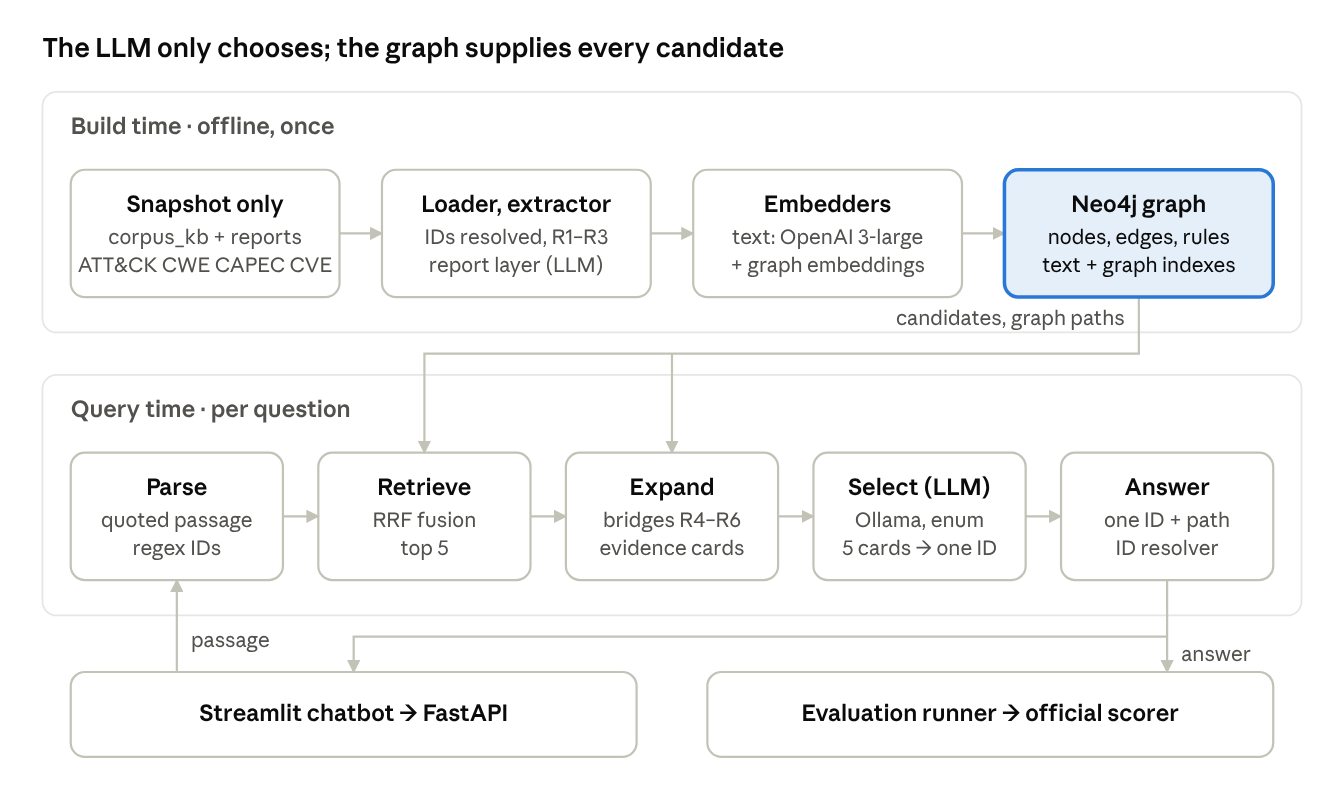
\includegraphics[width=0.86\textwidth]{architecture.png}
\caption{System architecture. Build time turns the CTIConnect snapshot into a validated Neo4j graph (rules R1--R3, the LLM report layer, text embeddings; GDS scores and provenance are written onto it). At query time the graph supplies five candidates and their evidence cards, Llama-3-8B chooses one under an enum constraint, and the answer returns with its graph paths.}
\label{fig:arch}
\end{figure*}

The graph is a labelled property graph in Neo4j 5.26 built only from CTIConnect's \texttt{corpus\_kb} snapshot (pinned commit \id{554797d}, snapshot date 2025-09-01) and its 321 report summaries. Fig.~\ref{fig:arch} shows where it sits in the system and Fig.~\ref{fig:schema} its schema.

\subsection{Node labels and relationship types}

Table~\ref{tab:nodes} lists the node labels. Identifiers are the canonical keys of each source taxonomy, enforced by uniqueness constraints, so every answer the system can give is a node the loader wrote from an official record. Table~\ref{tab:rels} lists the relationship types with their derivation; the counts match the Python derivation of the same snapshot and CTIFoundry's counts for it (CTIFoundry reports 1,214 and 272 CAPEC links because three CAPEC records list a link twice).

\begin{table}[t]
\caption{Node labels}
\label{tab:nodes}
\centering
\footnotesize
\begin{tabular}{@{}l r L{3.55cm}@{}}
\toprule
Label (key) & Nodes & Content \\
\midrule
AttackTechnique (\id{T1059.001}) & 1,076 & title, tactics, platforms, detection advice \\
Tactic (name) & 19 & from \texttt{kill\_chain\_phases} \\
CWE (\id{CWE-79}) & 1,342 & title, consequences, mitigations (412 empty) \\
CAPEC (\id{CAPEC-66}) & 615 & name, attack-language description \\
CVE (\id{CVE-2021-...}) & 2,751 & description; labelled CWE examples \\
ThreatReport (\id{BLOG-10}) & 321 & title, URL, publication date \\
ReportChunk (\id{BLOG-10\#0}) & 650 & text with character offsets \\
ReportBehavior & 3,512 & verbatim attacker-behavior phrase \\
Source & 3 & provenance records (Sec.~\ref{sec:props}) \\
\bottomrule
\end{tabular}
\end{table}

\begin{table}[t]
\caption{Relationship types (all directed)}
\label{tab:rels}
\centering
\footnotesize
\begin{tabular}{@{}l r l l@{}}
\toprule
Type & Edges & Method & Derived from \\
\midrule
SUBTECHNIQUE\_OF & 518 & derived & ID pattern \\
REPLACED\_BY & 103 & derived & retired-ID rule R2 \\
IN\_TACTIC & 1,374 & asserted & kill-chain phases \\
EXPLOITS\_WEAKNESS & 1,212 & asserted & CAPEC $\rightarrow$ CWE \\
MAPS\_TO\_TECHNIQUE & 271 & asserted & CAPEC $\rightarrow$ ATT\&CK \\
HAS\_WEAKNESS & 3,286 & asserted & NVD weaknesses \\
HAS\_CHUNK & 650 & segmented & chunking \\
HAS\_BEHAVIOR & 3,512 & segmented & verbatim span \\
GROUNDS & 3,512 & extracted & LLM, validated \\
\bottomrule
\end{tabular}
\end{table}

\begin{figure}[t]
\centering
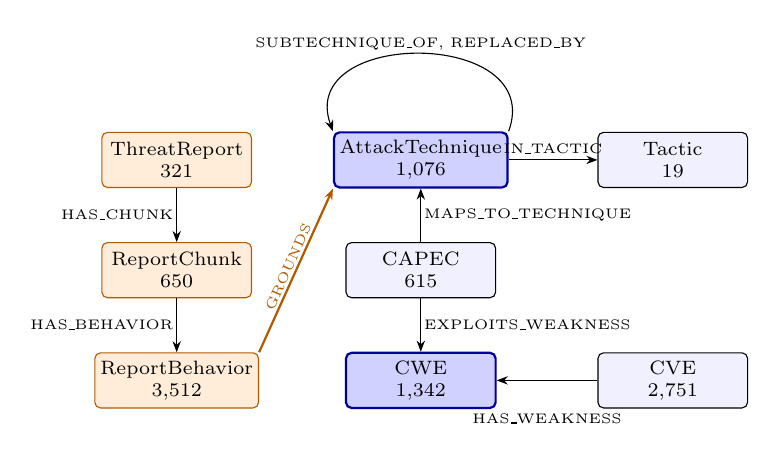
\begin{tikzpicture}[
  font=\scriptsize,
  box/.style={draw, rounded corners=2pt, align=center, minimum width=1.9cm, minimum height=0.7cm, inner sep=2pt},
  kb/.style={box, fill=blue!6},
  tgt/.style={box, fill=blue!18, draw=blue!60!black, thick},
  rep/.style={box, fill=orange!15, draw=orange!70!black},
  lab/.style={font=\tiny, inner sep=1pt},
  >={Stealth[length=4pt]}]
\node[rep] (rpt) at (0,0) {ThreatReport\\321};
\node[rep] (chk) at (0,-1.4) {ReportChunk\\650};
\node[rep] (beh) at (0,-2.8) {ReportBehavior\\3,512};
\node[tgt] (tec) at (3.1,0) {AttackTechnique\\1,076};
\node[kb]  (cap) at (3.1,-1.4) {CAPEC\\615};
\node[tgt] (cwe) at (3.1,-2.8) {CWE\\1,342};
\node[kb]  (tac) at (6.3,0) {Tactic\\19};
\node[kb]  (cve) at (6.3,-2.8) {CVE\\2,751};
\draw[->] (rpt) -- node[lab, left] {HAS\_CHUNK} (chk);
\draw[->] (chk) -- node[lab, left] {HAS\_BEHAVIOR} (beh);
\draw[->, orange!70!black, thick] (beh.north east) -- node[lab, sloped, above, pos=0.5] {GROUNDS} (tec.south west);
\draw[->] (tec) -- node[lab, above=1pt] {IN\_TACTIC} (tac);
\draw[->] (cap) -- node[lab, right] {MAPS\_TO\_TECHNIQUE} (tec);
\draw[->] (cap) -- node[lab, right] {EXPLOITS\_WEAKNESS} (cwe);
\draw[->] (cve) -- node[lab, below=11pt] {HAS\_WEAKNESS} (cwe);
\draw[->] (tec.north east) to[out=70, in=110, looseness=1.6] node[lab, above] {SUBTECHNIQUE\_OF, REPLACED\_BY} (tec.north west);
\end{tikzpicture}
\caption{Graph schema with node counts. Dark blue: answer targets; orange: the LLM report layer.}
\label{fig:schema}
\end{figure}

\subsection{Edge properties: provenance, timestamps, confidence}\label{sec:props}

Every relationship records where it came from and how much to trust it:
\begin{itemize}
\item \texttt{source}: the id of a \texttt{Source} node, which holds the snapshot's repository, pinned commit and date, or the report-layer build (model, prompt, extraction date, counts).
\item \texttt{method}: \emph{asserted} (stated in a source record), \emph{derived} (a deterministic rule), \emph{segmented} (report chunking) or \emph{extracted} (the LLM), with a free-text \texttt{derivation}.
\item \texttt{loaded\_at} (load timestamp) and \texttt{confidence}: 1.0 for asserted, derived and segmented edges; for extracted edges, the audited precision of the edge's confidence tier (Section~\ref{sec:conf}).
\end{itemize}
Some types carry more. \texttt{HAS\_WEAKNESS} keeps NVD's weakness type (1,882 Primary, 1,404 Secondary). \texttt{MAPS\_TO\_TECHNIQUE} keeps CAPEC's own name for the mapped technique and its agreement with the current ATT\&CK title, which flags stale mappings (one of 271: CAPEC-662 ``Man in the Browser'' now points to T1185 ``Browser Session Hijacking''). \texttt{GROUNDS} keeps the model, prompt, extraction date, the validation checks passed, the soft signals behind its confidence and its tier, and \texttt{HAS\_BEHAVIOR} keeps the behavior's character span in its report; all 3,512 spans resolve to the exact report text. Indexes cover identifier uniqueness, normalized titles, a relationship index on \texttt{GROUNDS.confidence}, and five 3,072-dimensional cosine vector indexes over technique, CWE, CAPEC, CVE and behavior embeddings (text-embedding-3-large).

\subsection{Reference ontologies and the RDF/OWL versus LPG decision}

Labels follow the source vocabularies one to one: ATT\&CK techniques, sub-techniques and tactics~\cite{attack}, CWE, CAPEC and CVE, keyed by their official identifiers. In STIX 2.1, ATT\&CK techniques and CAPEC patterns are both represented as \emph{attack-pattern} objects (ATT\&CK is distributed that way) and CVEs as \emph{vulnerability} objects; we keep separate labels because their identifier spaces and their roles in the two tasks differ (a technique or CWE is an answer, a CAPEC or CVE is evidence).

We chose a labelled property graph over RDF/OWL~\cite{hogan2021kg} for three reasons. First, the properties that matter here (confidence, character spans, provenance) belong to edges, which a property graph stores directly and RDF needs reification or RDF-star for. Second, the workload is traversal, vector search and graph algorithms, all native to Neo4j and its GDS library. Third, the inference needed is small and deterministic (sub-technique hierarchy, retired identifiers, domain), computed once at load time as rules R1--R3; no OWL reasoning is required, so the n10s RDF plugin is not used. The cost is weaker interoperability with semantic-web tooling. Within the approved scope we did not build an RDF export.

\subsection{What is excluded, and why}

To stay comparable with CTIConnect, the graph uses no outside data (no MITRE STIX bundles, CWE XML or NVD lookups: a cited CVE's NVD entry, for example, names the answer) and none of the benchmark's \texttt{construction/} files, whose seeds generated the questions. One consequence is that the graph has no CWE parent--child hierarchy; Section~\ref{sec:gds} measures what that costs. Attributes that would narrow the answer space (ATT\&CK domain, retired status) are shown on evidence cards but never used as filters: on the development split such filters raised recall only by assuming what the answers look like.

\section{Extraction and Ingestion Architecture}\label{sec:extraction}

\subsection{Structured ingestion and normalization}

A Python loader reads the four snapshot files (fetched at the pinned commit with checksum verification) and writes nodes and edges with batched \texttt{UNWIND ... MERGE} statements through the Neo4j driver. Normalization covers identifier formats (CWE identifiers upper-cased; CAPEC's ATT\&CK taxonomy entries prefixed with \id{T}; CVE weakness values kept only if the CWE exists), duplicate links (three CAPEC records list a link twice and are counted once), titles (a normalized lowercase key for lookup) and three snapshot-derived rules: R1 assigns each technique a domain (Enterprise, Mobile, ICS) from its platforms and identifier prefix; R2 finds 103 retired Enterprise parent-level identifiers whose title equals a sub-technique's and links them with \texttt{REPLACED\_BY}; R3 derives the hierarchy from the identifier pattern and tactics from kill-chain phases. The loader checks every edge count against the in-memory derivation, then embeds one text view per searchable node (title plus record content for techniques and CWEs, name plus description for CAPEC, description for CVE, the phrase for behaviors), cached on disk. A full load takes about 30 seconds.

\subsection{Unstructured extraction: the report layer}

Following CTIFoundry~\cite{ctifoundry}, each of the 321 report summaries is split at clause boundaries into chunks of 200--900 characters with exact offsets (650 chunks). Each chunk is sent once to the extractor with CTIFoundry's TTP-grounding prompt, its tactic list filled from the snapshot:

\begin{quote}\footnotesize\ttfamily
Extract MITRE ATT\&CK techniques from this CTI report chunk. [...] List every ATTACKER behavior in the chunk that corresponds to a real ATT\&CK technique. For each: "behavior" = the verbatim phrase; "technique\_id" = the ATT\&CK id, most specific you are confident in; "technique\_name" = official name. STRICT rules: Attacker techniques ONLY. EXCLUDE defenses/mitigations [...] Do NOT invent ids.
\end{quote}

\textbf{Schema enforcement.} Decoding is constrained to a strict JSON schema generated from the Pydantic model \texttt{ExtractionReply}: a list of records with required \texttt{behavior}, \texttt{technique\_id} (pattern \verb|^T\d{4}(\.\d{3})?$|) and \texttt{technique\_name}, and no additional properties. Each returned record is then validated twice by Pydantic: \texttt{ExtractedTTP} checks shape and identifier format, and \texttt{GroundedBehavior}, validated with the chunk as context, rejects identifiers absent from the snapshot and phrases that do not occur verbatim in the chunk (zero fabrication by construction). The committed layer was extracted with gpt-5.4-mini at the provider's default temperature, before constrained decoding was added; re-validating its 3,741 cached records with the Pydantic path reproduces it byte for byte: 0 schema failures, 6 unknown identifiers and 223 non-verbatim phrases dropped, 3,512 kept, covering 353 techniques and 627 of 650 chunks.

The layer never answers a question from its own source: 0 of 73 development passages occur verbatim in their report's summary, and SGS always excludes the question's own report. It serves as labelled examples of how reports word each technique.

\subsection{Confidence tiers and their audit}\label{sec:conf}

The hard checks keep only grounded records but cannot tell a right identifier from a wrong one. Two soft signals sort the 3,512 \texttt{GROUNDS} edges into tiers: the agreement (difflib ratio) between the technique name the model wrote and the official title of the identifier it gave, which catches wrong identifiers, and the rank of the technique among all 1,076 for the behavior phrase alone by embedding similarity, which catches context-dependent mappings. We drew a stratified sample of 25 edges per tier (seed 6338) and labelled each correct if the identifier is a right ATT\&CK mapping for the behavior in its chunk. The tier's precision becomes the confidence of every edge in it (Table~\ref{tab:audit}).

\begin{table}[t]
\caption{Report-layer confidence tiers and audited precision}
\label{tab:audit}
\centering
\footnotesize
\begin{tabular}{@{}l l r r@{}}
\toprule
Tier & Rule & Edges & Precision [95\% CI] \\
\midrule
supported & agreement $\ge$ 0.6, rank $\le$ 50 & 2,488 & 0.76 [0.57, 0.89] \\
context & agreement $\ge$ 0.6, rank $>$ 50 & 934 & 0.24 [0.12, 0.43] \\
conflict & agreement $<$ 0.6 & 90 & 0.32 [0.17, 0.52] \\
\midrule
all & tier-weighted & 3,512 & 0.61 \\
\bottomrule
\end{tabular}
\end{table}

The estimated precision of the layer is 0.61. Errors are mostly sibling sub-techniques (HTML smuggling mapped to \id{T1027.016} instead of \id{T1027.006}; Java mapped to \id{T1059.006}, Python), vague phrases mapped to a technique (``initial access'' to \id{T1190}), and defender actions read as attacker behavior. Name disagreement is not always an error: some reflect ATT\&CK renames (\id{T1574.001} is now ``DLL''; extortion falls under \id{T1657}).

\subsection{A local extractor under the same schema}

To test whether the local model could build the layer itself, we ran the same prompt and schema with Llama-3-8B-Instruct (fp16, Ollama, temperature 0) on 40 sampled chunks. Constrained decoding removed malformed output entirely (0 schema failures in 209 records), but 29\% of records failed grounding (58 non-verbatim, 3 unknown identifiers, against 6\% for gpt-5.4-mini), and agreement with the gpt-5.4-mini layer on (chunk, technique) pairs was F1 0.14 exactly and 0.23 at the technique-family level, at 12.3 s per chunk. The committed layer therefore stays the gpt-5.4-mini build; the 8B model is used only to answer.

\section{Graph Data Science and Reasoning}\label{sec:gds}

\subsection{Projection and algorithms}

A Cypher script (\texttt{gds.cypher}) projects only the knowledge-base layer (5,803 nodes, 6,764 relationships); the report layer is left out so no score carries information from the reports the questions come from. On the undirected projection it runs degree centrality, weakly connected components (WCC), Louvain community detection~\cite{blondel2008louvain} (single-threaded for reproducible community identifiers) and betweenness centrality~\cite{brandes2001}; PageRank~\cite{page1999pagerank} runs on the stored direction (damping 0.85; it converged in 4 iterations), so a node ranks high when much of the knowledge base points at it. Each result is written back as a node property. All algorithms together run in under one second. Fig.~\ref{fig:cypher} shows the core calls and one reasoning query.

\begin{figure}[t]
\scriptsize
\begin{verbatim}
CALL gds.graph.project('kb',
  ['AttackTechnique','Tactic','CWE','CAPEC','CVE'],
  {SUBTECHNIQUE_OF: {orientation:'UNDIRECTED'},
   IN_TACTIC: {orientation:'UNDIRECTED'}, ...});
CALL gds.louvain.write('kb',
  {writeProperty:'community', concurrency:1})
YIELD communityCount, modularity;
CALL gds.pageRank.write('kb_directed',
  {writeProperty:'pagerank', dampingFactor:0.85});

// R4, the CAPEC bridge, for a passage vector $v
MATCH (c:CAPEC)
WITH c, vector.similarity.cosine(c.embedding, $v) AS s
ORDER BY s DESC LIMIT 10
MATCH (c)-[:EXPLOITS_WEAKNESS]->(w:CWE)
RETURN w.id, sum(2*s - 1) AS score   // Neo4j: (1+cos)/2
ORDER BY score DESC;
\end{verbatim}
\caption{Excerpts of \texttt{gds.cypher} and of the Cypher form of rule R4.}
\label{fig:cypher}
\end{figure}

\subsection{Topology}

\begin{table}[t]
\caption{Degree by label on the knowledge-base projection}
\label{tab:degree}
\centering
\footnotesize
\begin{tabular}{@{}l r r r r r@{}}
\toprule
Label & Nodes & Mean & Median & Max & Isolated \\
\midrule
AttackTechnique & 1,076 & 2.68 & 2 & 20 & 0 \\
Tactic & 19 & 72.3 & 53 & 304 & 0 \\
CWE & 1,342 & 3.35 & 0 & 317 & 891 \\
CAPEC & 615 & 2.41 & 1 & 17 & 131 \\
CVE & 2,751 & 1.19 & 1 & 4 & 0 \\
\bottomrule
\end{tabular}
\end{table}

Table~\ref{tab:degree} shows the degree distribution. Tactics are hubs (defense-evasion has 304 techniques). Two thirds of CWEs (891 of 1,342) are isolated: without a CWE hierarchy, a CWE is connected only if a CVE or CAPEC points at it. WCC finds 1,116 components: one giant component of 4,451 nodes (1,066 techniques, 344 CWEs, 459 CAPECs, 2,565 CVEs) and mostly singletons.

\textbf{Centrality.} CWE PageRank tracks how often CVEs are labelled with a weakness: \id{CWE-79} (37.7), \id{CWE-89} (21.7), \id{CWE-74} (13.4), \id{CWE-200}, \id{CWE-787}. Technique leaders are \id{T1195}, \id{T1027}, \id{T1036} and \id{T1218}. CAPEC nodes have only outgoing edges, so their PageRank is flat; betweenness ranks them instead and identifies the bridges between the vulnerability side and the ATT\&CK side: \id{CWE-20}, \id{CWE-79}, \id{CWE-200} and \id{CAPEC-13}, \id{CAPEC-60}, \id{CAPEC-76}.

\textbf{Communities.} Louvain finds 1,149 communities with modularity 0.864 over four levels. The largest group CVEs around one weakness family (cross-site scripting, 384 nodes; input validation, 361; SQL injection, 278; out-of-bounds reads, 231) or techniques around tactics (persistence and privilege escalation, 327; defense evasion, 228). As a check of semantic coherence, 79.4\% of techniques fall in a community whose dominant tactic is one of their own, although tactics were only one of six relationship types in the projection.

\textbf{Paths.} The CVE $\rightarrow$ CWE $\leftarrow$ CAPEC $\rightarrow$ technique bridge links the two tasks: 260 CWEs have CVE examples, 336 have CAPEC patterns and 149 reach at least one technique through CAPEC; 189 techniques have a CAPEC. The graph holds 7,866 such paths. A Dijkstra shortest path, for example, connects \id{CVE-2020-12790} $\rightarrow$ \id{CWE-74} $\rightarrow$ \id{CAPEC-13} $\rightarrow$ \id{T1562.003} in three hops.

\subsection{Rule-based reasoning: snapshot bridges}

Beyond R1--R3, three rules run per question as a vector search followed by one-hop aggregation over the graph. With unit-normalized embeddings and similarity $s(q,x)$, a bridge scores a target $t$ by the records that point to it:
\begin{equation}
S_B(t) = \sum_{x \in \mathrm{top}_{n_B}(B,\,q),\; x \to t} s(q, x),
\end{equation}
for R4, CAPEC patterns ($n=10$, via \texttt{EXPLOITS\_WEAKNESS}); R5, CVE examples ($n=20$, via \texttt{HAS\_WEAKNESS}); and R6, report behaviors from other reports ($n=30$, via \texttt{GROUNDS}). Rankings are fused by reciprocal-rank fusion~\cite{cormack2009rrf}, $\mathrm{RRF}(v)=\sum_r 1/(60+\mathrm{rank}_r(v))$. ATA fuses dense retrieval over all techniques (question and passage) with R6; VCA fuses dense retrieval over CWEs with R4 and R5. Each bridge is also a single Cypher query; run end to end through Neo4j, SGS scores F1 0.452 against 0.466 in memory, a one-question difference caused by near-ties between 32-bit and 64-bit similarities. Table~\ref{tab:rules} summarizes the six rules and Table~\ref{tab:components} what each ranking contributes alone.

\begin{table}[t]
\caption{Snapshot-derived rules and how SGS uses them}
\label{tab:rules}
\centering
\footnotesize
\begin{tabular}{@{}L{1.45cm} L{2.35cm} L{3.55cm}@{}}
\toprule
Rule & Inference & Use and development-split evidence \\
\midrule
R1 Domain & Enterprise, Mobile or ICS from platforms and ID & shown on cards, never a filter (a filter raised ATA recall@5 0.57 to 0.60 only by assuming the answer space) \\
R2 Retired ID & parent ID with a sub-technique's title & stored; excluding them is an ablation only \\
R3 Hierarchy, tactics & ID pattern, kill-chain phases & tactics on cards; tactic-first narrowing lowered recall@5 0.57 to 0.50 (the model names the tactic 50\% of the time) \\
R4 CAPEC bridge & passage $\approx$ CAPEC $\rightarrow$ CWE & VCA candidates; CAPEC name on cards \\
R5 CVE vote & passage $\approx$ CVE $\rightarrow$ CWE & VCA candidates; closest CVE on cards \\
R6 Report vote & passage $\approx$ behavior $\rightarrow$ technique & ATA candidates; two examples on cards \\
\bottomrule
\end{tabular}
\end{table}

\begin{table}[t]
\caption{Recall@5 of each ranking alone (development split)}
\label{tab:components}
\centering
\footnotesize
\begin{tabular}{@{}l r r@{}}
\toprule
Ranking & ATA (1,076 techniques) & VCA \\
\midrule
Dense, full question & 0.57 & 0.40 \\
Dense, quoted passage & 0.47 & 0.21 \\
R6 report-example vote & 0.53 & -- \\
R4 CAPEC bridge & 0.03 & 0.35 \\
R5 CVE vote & -- & 0.26 \\
BM25, passage (dropped) & 0.30 & 0.16 \\
\midrule
Fused (SGS) & 0.63 & 0.65 \\
\bottomrule
\end{tabular}
\end{table}

\subsection{GDS outputs and graph embeddings as retrieval signals}

Candidate recall caps every method: the small model cannot choose an answer it never sees. We therefore tested graph signals as rankers on the development split, without the LLM. The \emph{PageRank prior} adds $\beta\,\tilde p_v$, the log PageRank scaled to $[0,1]$ within the target label; the \emph{community vote} adds $\gamma$ times the share of the question's ten nearest knowledge-base nodes, weighted by similarity, that lie in the candidate's Louvain community. We also tested two graph embeddings: \emph{propagated text embeddings}, a training-free GraphSAGE/APPNP-style smoothing~\cite{hamilton2017graphsage,gasteiger2019appnp}
\begin{equation}
H^{(k+1)} = (1-\alpha)X + \alpha D^{-1}AH^{(k)},
\end{equation}
with the question's own report edges removed, and node2vec~\cite{grover2016node2vec} structural embeddings anchored on the question's nearest nodes. Table~\ref{tab:signals} gives the results.

\begin{table}[t]
\caption{Candidate recall on the development split (no LLM)}
\label{tab:signals}
\centering
\footnotesize
\begin{tabular}{@{}l r r r r@{}}
\toprule
& \multicolumn{2}{c}{ATA} & \multicolumn{2}{c}{VCA} \\
Ranking & @1 & @5 & @1 & @5 \\
\midrule
Text embedding of the question & 0.40 & 0.57 & 0.12 & 0.40 \\
SGS candidates (dense + R4--R6) & 0.33 & 0.63 & 0.16 & 0.65 \\
\quad + PageRank prior (RRF) & 0.43 & 0.77 & 0.35 & 0.63 \\
\quad + PageRank and community (RRF) & 0.40 & 0.77 & 0.33 & 0.65 \\
Propagated text embeddings & 0.40 & 0.80 & 0.47 & 0.70 \\
node2vec + text (best) & -- & 0.60 & -- & 0.56 \\
\bottomrule
\end{tabular}
\end{table}

PageRank acts as a base-rate prior: the median gold CWE sits at the 95.5th PageRank percentile (techniques: 70th), and every gold answer has at least one edge even though 66\% of CWEs have none. A leak check found no development passage duplicating a knowledge-base CVE (median best cosine 0.48, none above 0.9). Graph signals mostly sharpen the top of the list (VCA recall@1 0.16 to 0.35), and propagated embeddings give the best recall@5 on both tasks. Weights were chosen on the same split, so these gains are optimistic, and feeding these candidates to the LLM is future work; the frozen SGS configuration evaluated below does not use them.

\section{LLM Integration and GraphRAG}\label{sec:graphrag}

\subsection{Snapshot-Guided Selection}

SGS divides the work: the graph proposes and explains candidates, and the small model only chooses. For each question it (1) extracts the quoted passage and any identifiers by regular expression; (2) retrieves the top five candidates with the fused rankings of Section~\ref{sec:gds}; (3) builds one evidence card per candidate from graph paths only; and (4) asks Llama-3-8B-Instruct to choose. ATA cards hold the title, tactics, platforms, first sentence of detection advice and the two report-layer sentences closest to the passage, never from its own report; VCA cards hold the title, consequences, a related CAPEC pattern and the closest CVE example. A real card:

\begin{quote}\footnotesize\ttfamily
T1071.003 | Mail Protocols | tactics: command-and-control | platforms: Linux, macOS, Windows, Network Devices | detection: [...] | report examples: "...the email-based NightClub (SMTP/IMAP C2) and its 2020-onward successor Disco..."
\end{quote}

The prompt, under the system message ``You are a cyber threat intelligence analyst.'', is:

\begin{quote}\footnotesize\ttfamily
You are mapping a threat-report passage to \{MITRE ATT\&CK techniques | CWE weaknesses\}.\\
Passage: "\{passage\}"\\
Candidates:\\
\{cards\}\\
Choose the ONE candidate that best describes the behavior in the passage. Judge by what each candidate means, not by shared words. Return JSON with its id.
\end{quote}

\noindent Decoding is constrained to a JSON schema whose only field is an enum of the five candidate identifiers, at temperature 0, and the reply is re-validated by a Pydantic model of the same enum. An identifier outside the list is therefore impossible. For VCA, the list is shown in its five cyclic rotations and the majority wins (ties go to the better retrieval rank), which cancels position bias. The answer text holds exactly one identifier and its title, because the official scorer counts every identifier it finds; an optional explanation step is scrubbed of all other identifiers.

\textbf{Tested and dropped.} Several alternatives lost on the development split: showing ten candidates instead of five lowered selection accuracy even when the gold was listed (ATA 0.50 vs 0.59, VCA 0.43 vs 0.54); a pairwise tournament in both orders reached at most 0.40 on either task with up to eight calls; a rotation vote for ATA was no better than one call; and narrowing ATT\&CK candidates to the model's guessed tactic hurt recall (Table~\ref{tab:rules}). A separate fact-checking layer was unnecessary: once candidates are shown, the model's identifier and title contradict the graph in 1 of 12 sampled pairs, against 11 of 21 closed-book.

\subsection{Graph citations and provenance tracking}

Every answer carries the graph paths behind the chosen identifier, kept in the trace and the API response rather than the scored text. A \emph{report} citation is a path \texttt{ThreatReport} $\rightarrow$ \texttt{ReportChunk} $\rightarrow$ \texttt{ReportBehavior} $\rightarrow$ technique with the behavior's character span, tier and \texttt{GROUNDS} confidence; \emph{capec} and \emph{cve} citations are bridge paths with their similarity to the passage and, for CVEs, NVD's Primary or Secondary tag; \emph{taxonomy} citations are tactic and hierarchy edges. Each citation records whether the model saw it on the card, and carries a Cypher \texttt{MATCH} that returns exactly that path. For development question \texttt{ata-012} (Androxgh0st abusing SMTP), SGS answers \id{T1071.003} and cites
\texttt{BLOG-210} $\rightarrow$ \texttt{BLOG-210\#0} $\rightarrow$ ``the email-based NightClub (SMTP/IMAP C2)'' $\rightarrow$ \id{T1071.003}, characters 195--235 of a different report, confidence 0.76.

\subsection{Interfaces}

A service layer turns an \texttt{AttributionRequest} into an \texttt{AttributionResponse} (answer, explanation, candidates and cards, votes, LLM calls, citations, latency). A FastAPI app exposes it (\texttt{POST /attribute}, \texttt{GET /graph/\{id\}} for an answer node's PageRank and Louvain community, \texttt{POST /verify} for live path checks, which accepts a citation path rather than raw Cypher and runs a parameterized, schema-checked query). A Streamlit chatbot shows the answer, timings and tabs for citations with a ``verify in Neo4j'' button, the cited subgraph, the candidates and cards, the answer's graph analytics and every LLM call.

\section{Evaluation and Discussion}\label{sec:eval}

\subsection{Setup}

The 379 attribution questions (ATA 160, VCA 219; one gold identifier each) are split by source report (seed 13) into a development split of 73 questions from 29 reports (30 ATA, 43 VCA) and a test split of 306. All design decisions were made on the development split, and all results below are on it; the test split has not been run and is reserved for future work. Every method uses Llama-3-8B-Instruct at fp16 (\texttt{llama3:8b-instruct-fp16}, Ollama 0.35.0, temperature 0) and text-embedding-3-large, and is scored by CTIConnect's official identifier F1, vendored unmodified. A failed call scores zero rather than being dropped. Baselines are CTIConnect's closed-book (CB) and vanilla RAG (VR, top-5 knowledge-base records retrieved by the question), with their prompts verbatim. Two pairs of ATA questions are identical but have different gold answers, so the ATA ceiling is 0.988. Significance uses paired bootstrap intervals~\cite{efron1993} (10,000 resamples) and McNemar's exact test~\cite{mcnemar1947} on exact match.

\subsection{Response accuracy}

\begin{table}[t]
\caption{F1 on the development split (Llama-3-8B fp16)}
\label{tab:acc}
\centering
\footnotesize
\begin{tabular}{@{}l r r r@{}}
\toprule
Method & ATA (30) & VCA (43) & Overall \\
\midrule
CB, closed-book & 0.033 & 0.132 & 0.091 \\
VR, vanilla RAG & 0.289 & 0.233 & 0.256 \\
Cards, one listwise call & 0.33 & 0.35 & 0.34 \\
\quad + report examples (R6) & 0.43 & 0.35 & 0.38 \\
\quad + VCA rotation vote = \textbf{SGS} & \textbf{0.433} & \textbf{0.488} & \textbf{0.466} \\
SGS, candidates from Neo4j & 0.433 & 0.465 & 0.452 \\
\midrule
\multicolumn{4}{@{}l}{\emph{CTIConnect reported, Llama-3-8B, all 379 questions:}} \\
VR / DtR & 0.28 / 0.28 & 0.22 / 0.40 & -- \\
\bottomrule
\end{tabular}
\end{table}

Table~\ref{tab:acc} gives F1 with the ablation ladder. SGS reaches 0.466 against 0.256 for vanilla RAG on the same questions. The paired difference is +0.210 (95\% CI [+0.082, +0.338]); by task it is +0.256 [+0.093, +0.419] for VCA and +0.144 [$-0.067$, +0.356] for ATA, where 30 questions do not resolve it. On exact match SGS is right where VR is wrong on 24 questions and the reverse on 5 (McNemar $p=0.0005$). Scoring answers as (report, predicate, identifier) triples against 69 gold triples gives triple F1 0.511 for SGS, 0.253 for VR and 0.130 for CB. The ladder attributes the gain: graph candidates and cards (+0.08 over VR), report-layer examples for ATA (+0.10 on ATA) and the rotation vote for VCA (+0.14 on VCA). With one question worth 0.03 (ATA) or 0.02 (VCA), single-question differences between configurations are noise.

\subsection{Hallucination}

We count, for each answer, whether it names an identifier absent from the snapshot (fabricated), names none, or names several (hedged; the scorer counts all of them). Table~\ref{tab:hall} shows that retrieval alone removes fabricated identifiers but not hedging, and that SGS removes both by construction. Closed-book fabricates in 23\% of ATA answers, for example the nonexistent \id{T1193.001} three times.

\begin{table}[t]
\caption{Identifier hallucination, share of the 73 answers}
\label{tab:hall}
\centering
\footnotesize
\begin{tabular}{@{}l r r r@{}}
\toprule
Method & Fabricated ID & No ID & Hedged ($>$1 ID) \\
\midrule
CB, closed-book & 10\% (ATA 23\%) & 7\% & 11\% \\
VR, vanilla RAG & 0\% & 0\% & 23\% \\
SGS & 0\% & 0\% & 0\% \\
\bottomrule
\end{tabular}
\end{table}

\subsection{Faithfulness and provenance}

With its explanation step, SGS also scores higher than VR on RAGAS~\cite{es2024ragas} over the 20 evaluation queries (judge gpt-5.4-mini; contexts are exactly what each method showed the model): faithfulness 0.51 vs 0.46, answer relevancy 0.67 vs 0.60 and context recall 0.46 vs 0.39. Faithfulness near 0.5 reflects that the questions' extra asks (affected platforms, business consequences) are answered from the model's own knowledge, which the cards do not cover. For provenance, the 73 SGS answers carry 249 citations (79 report, 66 CAPEC, 58 CVE, 46 taxonomy); every answer has at least one evidence path, and all 249 Cypher queries return exactly one path from the live graph. Correct and wrong answers carry about as many evidence paths (2.71 vs 2.85), so citations make an answer checkable but do not by themselves indicate that it is right.

\subsection{Latency and extraction quality}

On the local Ollama, an ATA answer takes 4.0 s on average (one call) and a VCA answer 15.1 s (five rotation calls, at most 17.4 s); the LLM accounts for over 99\% of the time, while retrieval takes about 5 ms and building citations about 7 ms. Extraction quality is reported in Section~\ref{sec:extraction}: precision 0.61 from the stratified audit. Extraction recall was not measured, since the snapshot has no chunk-level labels; as a proxy, 29 of 30 development ATA gold techniques have at least one example from another report.

\subsection{Error analysis}

Table~\ref{tab:errors} splits the 39 wrong SGS answers by whether the gold identifier reached the model. Two thirds (26) are retrieval misses: the gold was not among the five candidates. When it was listed, the model chose it in 68\% of ATA and 75\% of VCA questions, and on VCA it was right three times when the gold was ranked fifth, which is the rotation vote at work. Two of the six ATA selection errors chose a sibling or parent of the gold technique. The VCA vote is also a usable confidence signal: unanimous answers (5 of 5 rotations) were correct in 10 of 16 questions, two-vote answers in 1 of 5.

\begin{table}[t]
\caption{Where SGS answers go wrong (development split)}
\label{tab:errors}
\centering
\footnotesize
\begin{tabular}{@{}l r r@{}}
\toprule
& ATA (30) & VCA (43) \\
\midrule
Correct & 13 & 21 \\
Gold not in the five candidates & 11 & 15 \\
Gold listed, another chosen & 6 & 7 \\
\midrule
Accuracy when the gold is listed & 0.68 & 0.75 \\
\bottomrule
\end{tabular}
\end{table}

\subsection{Discussion}

The results support the project's premise. A small model given the same knowledge as raw retrieved text (VR) improves over closed-book, but it still generates: it hedges, and it misreads identifiers. Moving generation into the graph, so that the model only compares five evidence cards, nearly doubles F1, and the evidence that matters most is relational: report wording from \emph{other} reports for ATA (R6) and CAPEC and CVE examples for VCA (R4, R5). The remaining errors are mostly retrieval misses (the gold is in the top five for 63\% of ATA and 65\% of VCA questions) and confusions between sibling sub-techniques, which the GDS and graph-embedding signals of Table~\ref{tab:signals} target.

\textbf{Limitations.} All results come from a 73-question split that also guided design, so they are optimistic and their intervals are wide; the 306-question test split remains to be run once. The audit behind the 0.61 extraction precision is a single first-pass annotation of 75 edges. The graph lacks a CWE hierarchy by design, which leaves two thirds of CWEs isolated. VCA latency is driven by the five-call vote. The scope approved for this course excludes entity-linking and multi-hop tasks, named-entity disambiguation of free-text mentions and an RDF export.

\textbf{Future work.} Run the held-out test split; feed the PageRank and propagated-embedding candidates to the LLM; weight report-layer votes by edge confidence; re-audit the extraction with a second annotator; and test smaller and newer open models.

\section{Conclusion}

Snapshot-Guided Selection shows that a knowledge graph built only from a benchmark's public snapshot can make a small local model a much better CTI attributor when the graph does the retrieving and the explaining and the model only chooses. On the development split it nearly doubles F1 over vanilla RAG, removes identifier hallucination, and returns every answer with provenance-rich graph citations that verify against the live graph. Graph Data Science shows the graph's structure (tactic-aligned communities, bridge nodes between vulnerabilities and techniques, and the cost of a missing CWE hierarchy) and points to the next gains in retrieval.

\begin{thebibliography}{99}

\bibitem{cticonnect}
Y.~Cheng, Y.~Liu, C.~Li, D.~Song, and P.~Gao, ``CTIConnect: A benchmark for retrieval-augmented LLMs over heterogeneous cyber threat intelligence,'' in \emph{Proc. KDD}, 2026, arXiv:2510.11974.

\bibitem{ctifoundry}
Y.~Cheng, C.~Li, Q.~Cui, L.~Wang, Y.~Chen, W.~Ding, and P.~Gao, ``CTIFoundry: An agent-native corpus scaffold for cyber threat intelligence,'' arXiv:2608.18613, 2026.

\bibitem{boyer2024}
A.~Boyer, E.~Dogdu, R.~Choupani, J.~S. Watson, D.~Sanchez, and A.~Ametu, ``Toward a unified cybersecurity knowledge graph: Leveraging ontologies and open data sources,'' in \emph{Recent Advances in Next-Generation Data Science}. Springer, 2024.

\bibitem{lewis2020rag}
P.~Lewis \emph{et~al.}, ``Retrieval-augmented generation for knowledge-intensive NLP tasks,'' in \emph{Proc. NeurIPS}, 2020.

\bibitem{edge2024graphrag}
D.~Edge, H.~Trinh, N.~Cheng, J.~Bradley, A.~Chao, A.~Mody, S.~Truitt, and J.~Larson, ``From local to global: A graph RAG approach to query-focused summarization,'' arXiv:2404.16130, 2024.

\bibitem{cormack2009rrf}
G.~V. Cormack, C.~L.~A. Clarke, and S.~B\"uttcher, ``Reciprocal rank fusion outperforms Condorcet and individual rank learning methods,'' in \emph{Proc. SIGIR}, 2009.

\bibitem{es2024ragas}
S.~Es, J.~James, L.~Espinosa-Anke, and S.~Schockaert, ``RAGAS: Automated evaluation of retrieval augmented generation,'' in \emph{Proc. EACL (System Demonstrations)}, 2024.

\bibitem{attack}
B.~E. Strom \emph{et~al.}, ``MITRE ATT\&CK: Design and philosophy,'' The MITRE Corporation, Tech. Rep., 2018.

\bibitem{hogan2021kg}
A.~Hogan \emph{et~al.}, ``Knowledge graphs,'' \emph{ACM Computing Surveys}, vol.~54, no.~4, 2021.

\bibitem{blondel2008louvain}
V.~D. Blondel, J.-L. Guillaume, R.~Lambiotte, and E.~Lefebvre, ``Fast unfolding of communities in large networks,'' \emph{J. Stat. Mech.}, P10008, 2008.

\bibitem{brandes2001}
U.~Brandes, ``A faster algorithm for betweenness centrality,'' \emph{J. Math. Sociol.}, vol.~25, no.~2, pp.~163--177, 2001.

\bibitem{page1999pagerank}
L.~Page, S.~Brin, R.~Motwani, and T.~Winograd, ``The PageRank citation ranking: Bringing order to the web,'' Stanford InfoLab, Tech. Rep., 1999.

\bibitem{hamilton2017graphsage}
W.~L. Hamilton, R.~Ying, and J.~Leskovec, ``Inductive representation learning on large graphs,'' in \emph{Proc. NeurIPS}, 2017.

\bibitem{gasteiger2019appnp}
J.~Gasteiger, A.~Bojchevski, and S.~G\"unnemann, ``Predict then propagate: Graph neural networks meet personalized PageRank,'' in \emph{Proc. ICLR}, 2019.

\bibitem{grover2016node2vec}
A.~Grover and J.~Leskovec, ``node2vec: Scalable feature learning for networks,'' in \emph{Proc. KDD}, 2016.

\bibitem{efron1993}
B.~Efron and R.~J. Tibshirani, \emph{An Introduction to the Bootstrap}. Chapman \& Hall, 1993.

\bibitem{mcnemar1947}
Q.~McNemar, ``Note on the sampling error of the difference between correlated proportions or percentages,'' \emph{Psychometrika}, vol.~12, no.~2, pp.~153--157, 1947.

\end{thebibliography}

\end{document}
